%!TEX root = presentazionelancia.tex
\section{Part II: Query Driven Stream Join (RDF)}
\begin{frame}[t]
\frametitle{Part II: Query Driven Stream Join (RDF)}
    \begin{center}
    	\includegraphics<1>[width=1\textwidth]{figs/semanticweb.jpg}
    \end{center}
\end{frame}




\begin{frame}
\frametitle{Outline}
	\begin{itemize}
		\item Introduction
		\item Query Decomposition and Data Partition
		\item Parallel and Distributed Query Plan
		\item Continuous Join
		\item Analysis
		\item Implementation
		\item Experiment Result
		\item Conclusion
	\end{itemize}
\end{frame}


\begin{frame}
\frametitle{Outline}
	\begin{itemize}
		\item Introduction
		\item \textcolor{blue!20}{Query Decomposition and Data Partition}
		\item \textcolor{blue!20}{Parallel and Distributed Query Planner}
		\item \textcolor{blue!20}{Continuous Join}
		\item \textcolor{blue!20}{Analysis}
		\item \textcolor{blue!20}{Implementation}
		\item \textcolor{blue!20}{Experiment Result}
		\item \textcolor{blue!20}{Conclusion}
	\end{itemize}
\end{frame}

\begin{frame}
\frametitle{Introduction --- RDF Data Model}
\begin{itemize}
\item \textbf{R}esource \textbf{D}escription \textbf{F}ramework is a data standard proposed by W3C
\item It aims at representing semantic data in a machine understandable manner.
\item This representation is used to describe semantic relations among data.
\item Data items are expressed as triples in form of <subject, predicate, object> (e.g. <Sophie, hasSister, Ray>)
\begin{itemize}
\item The subject of a triple indicates the resource that this triple is about.
\item The predicate refers to the property of the subject.
\item The object denotes to the projection value of the subject by the predicate.
\end{itemize}
\end{itemize}
\end{frame}

\begin{frame}
\frametitle{Introduction --- SPARQL Query Language}
\begin{itemize}
\item SPARQL is a W3C recommendation query language for querying RDF data.
\item The basic component of a SPARQL query is the  triple patterns.
\item A triple pattern is a special kind of triple where S, P and O can be either a literal or a variable.
\end{itemize}
\vspace{-0.2in}
\textbf{An Example (Triple Pattern Representation):}
\vspace{-0.2in}
    \begin{center}
    	\includegraphics<1>[width=1\textwidth]{figs/examplequery.png}
    \end{center}
\end{frame}

\begin{frame}
\frametitle{Introduction --- SPARQL Query Example}
\textbf{Graph Representation: }
\vspace{-0.25in}
    \begin{center}
    	\includegraphics<1>[width=0.6\textwidth]{figs/examplegraph.png}
    \end{center}
    \vspace{-0.25in}
\textbf{Relational Representation:}
\vspace{-0.25in}
    \begin{center}
    	\includegraphics<1>[width=0.5\textwidth]{figs/examplerelational.png}
    \end{center}
\end{frame}

\begin{frame}
\frametitle{Related Works --- 4 Types of Processing}
    \begin{center}
    	\includegraphics<1>[width=0.5\textwidth]{figs/type.png}
    \end{center}
\end{frame}

\begin{frame}
\frametitle{Partitioning Strategies}
\begin{itemize}
\item  Vertex Partitioning methods for graphs. 
\begin{itemize}
\item High overhead of loading big RDF graphs into the existing graph partitioner.
\item Requires the entire graph information in order to make decisions
\item Replication of the boundary of each partition in order to reduce the transmission of data
\end{itemize}
\item Hash Partitioning based on indexes
\end{itemize}
\end{frame}

\begin{frame}
\frametitle{Hash Partitioning --- Index}
    \begin{center}
    	\includegraphics<1>[width=0.7\textwidth]{figs/rdf3x.png}
    \end{center}
\end{frame}

\begin{frame}
\frametitle{Steps}
\begin{itemize}
\item Partition the RDF streams, and disperse these sub-streams to the nodes
\item Decompose the queries into sub-queries and assign these sub-queries to the appropriate nodes
\item Reply rapidly to the changes of data (the expiration of old data, and the update of new data), and return the results in real-time
\end{itemize}
\end{frame}


\begin{frame}
\frametitle{Outline}
	\begin{itemize}
		\item Introduction
		\item Query Decomposition and Data Partition
		\item \textcolor{blue!20}{Parallel and Distributed Query Planner}
		\item \textcolor{blue!20}{Continuous Join}
		\item \textcolor{blue!20}{Analysis}
		\item \textcolor{blue!20}{Implementation}
		\item \textcolor{blue!20}{Experiment Result}
		\item \textcolor{blue!20}{Conclusion}
	\end{itemize}
\end{frame}

\begin{frame}
\frametitle{Query Decomposition}
\textbf{Decomposition Strategy: }Divide the queries into triple patterns, send each triple pattern to some corresponding machines.
\begin{itemize}
\item It is simple, and does not require any complicated computations.
\item The sub-streams can be easily assigned to the sub-queries.
\item The performance or accuracy of this method does not depend on the index or replication of data.
\item Among the triples processed by a query, the number of different subjects or objects involved could be tens of thousands; But the number of triple patterns is a limited and  fixed number.
\end{itemize}

\end{frame}

\begin{frame}
\frametitle{Sub-Query Scheduling}
\textbf{Edge Coloring Method:}
\vspace{-0.2in}
    \begin{center}
    	\includegraphics<1>[width=0.5\textwidth]{figs/17.png}
    \end{center}
\end{frame}

\begin{frame}
\frametitle{Data Partitioning}
\textbf{Partitioning Strategy: }The triples with the same predicate will be assigned to the same nodes that hold the triple pattern with that same predicate.
\begin{itemize}
\item It does not require any index, and will not occupy more disk space.
\item It can quickly adapt to changes in data, and it does not require any re-partitioning on
the existing data when new data arrives or old data expires.
\item The number of different types of subjects and objects involved could be tens of thousands; But the number of different predicates is limited, and this number must be smaller than the number of triple patterns that compose this query.
\end{itemize}
\end{frame}


\begin{frame}
\frametitle{Outline}
	\begin{itemize}
		\item Introduction
		\item Query Decomposition and Data Partition
		\item Parallel and Distributed Query Planner
		\item \textcolor{blue!20}{Continuous Join}
		\item \textcolor{blue!20}{Analysis}
		\item \textcolor{blue!20}{Implementation}
		\item \textcolor{blue!20}{Experiment Result}
		\item \textcolor{blue!20}{Conclusion}
	\end{itemize}
\end{frame}

\begin{frame}
\frametitle{Problems to be solved to complete the decomposition and partitioning idea}
\begin{itemize}
\item The communication among nodes
\item The join of the intermediate results produced by each triple pattern
\item The order of sending and receiving information
\end{itemize}
\end{frame}

\begin{frame}
\frametitle{The communication among nodes --- Bloom Filter}
\begin{center}
    \includegraphics<1>[height=0.5\textwidth]{figs/bloomfilter_1.png}
    \includegraphics<2>[height=0.5\textwidth]{figs/bloomfilter_2.png}    	
    \includegraphics<3>[height=0.5\textwidth]{figs/bloomfilter_3.png}
    \includegraphics<4>[height=0.5\textwidth]{figs/bloomfilter_4.png}
    \includegraphics<5>[height=0.5\textwidth]{figs/bloomfilter_5.png}    	
    \includegraphics<6>[height=0.5\textwidth]{figs/bloomfilter_6.png}
    \includegraphics<7>[height=0.5\textwidth]{figs/bloomfilter_7.png}
    \includegraphics<8>[height=0.5\textwidth]{figs/bloomfilter_8.png}
\end{center}
\end{frame}

\begin{frame}
\frametitle{Bloom Filter --- Build and Probe}

\begin{itemize}

\item \textbf{Builder: } The triple patterns used to Build the Bloom Filter

\item \textbf{Prober: } The triple patterns used to Probe the Bloom Filter

\end{itemize}

\end{frame}

\begin{frame}
\frametitle{The join of the intermediate results --- Structure Based Rules}
\textbf{Rule 1: 1-Variable Join}
\vspace{0.3in}
\begin{columns}
\begin{column}{0.5\textwidth}
 	\includegraphics<1>[width=1\textwidth]{figs/2.png}
\end{column}
\begin{column}{0.5\textwidth}
 	\includegraphics<1>[width=1\textwidth]{figs/3.png}
\end{column}
\end{columns}
\end{frame}

\begin{frame}
\frametitle{The join of the intermediate results --- Structure Based Rules}
\textbf{Rule 2: 2-Variable Join}
\vspace{0.3in}
\begin{columns}
\begin{column}{0.5\textwidth}
 	\includegraphics<1>[width=1\textwidth]{figs/5.png}
\end{column}
\begin{column}{0.5\textwidth}
 	\includegraphics<1>[width=1\textwidth]{figs/6.png}
\end{column}
\end{columns}
\end{frame}

\begin{frame}
\frametitle{The join of the intermediate results --- Structure Based Rules}
\textbf{Rule 3: Multiple-Variable Join}
\vspace{0.3in}
\begin{columns}
\begin{column}{0.5\textwidth}
 	\includegraphics<1>[width=1\textwidth]{figs/8.png}
\end{column}
\begin{column}{0.5\textwidth}
 	\includegraphics<1>[width=1\textwidth]{figs/9.png}
\end{column}
\end{columns}
\end{frame}

\begin{frame}
\frametitle{The order of sending and receiving information}
\textbf{Rule 4: Query Topological Sort}
\begin{block}{Query Topological Sort}
\textbf{Query Topological Sort} is a topological sort for the query graphs, where the constant nodes on the graph have higher priority than the variable nodes at the same level.
\end{block}
\end{frame}

\begin{frame}
\frametitle{The order of sending and receiving information}
\textbf{Rule 4: Query Topological Sort}
\vspace{0.3in}
\begin{columns}
\begin{column}{0.5\textwidth}
 	\includegraphics<1>[width=1\textwidth]{figs/order.png}
\end{column}
\begin{column}{0.5\textwidth}
 	\includegraphics<1>[width=1\textwidth]{figs/querygraph.png}
\end{column}
\end{columns}
\textbf{Results: } $\{``O_4", ?S_2, ``S_1", ``O_3", ?O_2, ?O_1\}$
\end{frame}

\begin{frame}
\frametitle{Outline}
	\begin{itemize}
		\item Introduction
		\item Query Decomposition and Data Partition
		\item Parallel and Distributed Query Planner
		\item Continuous Join
		\item \textcolor{blue!20}{Analysis}
		\item \textcolor{blue!20}{Implementation}
		\item \textcolor{blue!20}{Experiment Result}
		\item \textcolor{blue!20}{Conclusion}
	\end{itemize}
\end{frame}

\begin{frame}
\frametitle{Continuous Join: Sliding Window + Sliding Bloom Filter}
    \begin{center}
    	\includegraphics<1>[width=0.8\textwidth]{figs/16.png}
    \end{center}
\end{frame}

\begin{frame}
\frametitle{Outline}
	\begin{itemize}
		\item Introduction
		\item Query Decomposition and Data Partition
		\item Parallel and Distributed Query Planner
		\item Continuous Join
		\item Analysis
		\item \textcolor{blue!20}{Implementation}
		\item \textcolor{blue!20}{Experiment Result}
		\item \textcolor{blue!20}{Conclusion}
	\end{itemize}
\end{frame}

\begin{frame}
\frametitle{Analysis}
\begin{itemize}
\item Bloom Filters
\item Dominating Parameters
\item Complexities
\end{itemize}
\end{frame}

\begin{frame}
\frametitle{Analysis About Bloom Filters --- False Positive Rate}
\begin{block}{Theorem 1}
Suppose that we use k hash functions to insert n elements into an m bits Bloom Filter, then the false positive rate p for a standard Bloom Filter is a function of n, m and k, and 
\begin{center}
p = $(1-e^{-\frac{nk}{m}})^k$
\end{center}
\end{block}
Idea: Balls and Bins
\end{frame}

\begin{frame}
\frametitle{Analysis About Bloom Filters --- Minimum False Positive Rate}
\vspace{-0.1in}
\begin{block}{Theorem 2}
The false positive $p$ reaches the minimum value, when 
\begin{center}
$e^{-\frac{nk}{m}}$ = $\frac{1}{2}$
\end{center}
At this extreme point, 
\begin{center}
k = ln2 $\times \frac{m}{n}$
\end{center}
And,
\begin{center}
p = $\frac{1}{2}^k$ = $2^{-ln2 \times \frac{m}{n}}$
\end{center}
\end{block}
\vspace{-0.25in}
Idea: p reaches the minimum value, when the derivation of p reaches 0.
\end{frame}



\begin{frame}
\frametitle{Outline}
	\begin{itemize}
		\item Introduction
		\item Query Decomposition and Data Partition
		\item Parallel and Distributed Query Planner
		\item Continuous Join
		\item Analysis
		\item Implementation
		\item \textcolor{blue!20}{Experiment Result}
		\item \textcolor{blue!20}{Conclusion}
	\end{itemize}
\end{frame}


\begin{frame}
\frametitle{Apache Storm}
    \begin{center}
    	\includegraphics<1>[width=0.8\textwidth]{figs/storm.png}
    	\includegraphics<2>[height=0.5\textwidth]{figs/storm1.png}
    \includegraphics<3>[height=0.5\textwidth]{figs/storm2.png} 
    \includegraphics<4>[height=0.5\textwidth]{figs/storm3.png}
    \end{center}
\end{frame}

\begin{frame}
\frametitle{Implementation}
\vspace{-0.1in}
\begin{center}
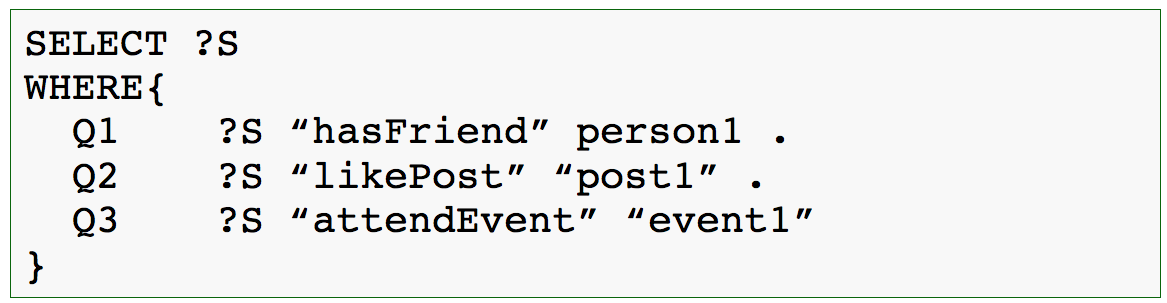
\includegraphics[width=0.5\textwidth]{figs/examplequery.png}
\end{center}
\vspace{-0.2in}
    \begin{center}
    	\includegraphics<1>[width=0.8\textwidth]{figs/implementation1.png}
    	\includegraphics<2>[width=0.8\textwidth]{figs/implementation2.png}
    \end{center}
\end{frame}


\begin{frame}
\frametitle{Outline}
	\begin{itemize}
		\item Introduction
		\item Query Decomposition and Data Partition
		\item Parallel and Distributed Query Planner
		\item Continuous Join
		\item Analysis
		\item Implementation
		\item Experiment Result
		\item \textcolor{blue!20}{Conclusion}
	\end{itemize}
\end{frame}

\begin{frame}
\frametitle{Experiment Setting}
\begin{itemize}
\item We evaluate the system on Grid 5000 4, with 11 nodes. Among them, one is reserved to be Nimbus, and the rest 10 nodes are used for computing. 

\item The Storm version is 1.0, and we only use one slot on each machine.

\item Apache Jena API is used for reading triples.
\end{itemize}

\end{frame}

\begin{frame}
\frametitle{Data sets}
\begin{itemize}
\item Synthetic data
\begin{itemize}
\item The RDF triples generated in Spouts are distributed to the nodes according to their predicate. 
\item Two sub-sets of data are generated. The  first sub-set contains only the results of the join, and the second one contains only the non-results of the join.
\end{itemize}
\item LUBM Data 
\begin{itemize}
\item LUBM has 14 queries, and we have tested query No.1, query No.3, and query No.4
\item It consists of a university domain. 
\item It is customizable and repeatable.
\end{itemize}
\end{itemize}
\end{frame}

\begin{frame}
\frametitle{Evaluations}
\textbf{Impacts: (x axis)}
\begin{itemize}
\item Sliding Window Size
\item Number of Generations
\end{itemize}
\textbf{Metrics: (y axis)}
\begin{itemize}
\item Execution Latency --- The difference between the time an element is generated and the time it is emitted as a result
\item Process Latency --- The difference between the time an element is generated and the time it begins to be processed
\item Data Transmitted
\item Accuracy
\end{itemize}
\end{frame}

\begin{frame}
\frametitle{Execution Lateny}
\vspace{-0.1in}
Sliding Window Size = 800 (1V)
\vspace{-0.2in}
    \begin{center}
    	\includegraphics<1>[width=0.7\textwidth]{figs/II_1V_EL.png}
    \end{center}
\end{frame}

\begin{frame}
\frametitle{Execution Latency}
\vspace{-0.1in}
Number of Generation = 6 (1V)
\vspace{-0.2in}
\begin{center}
    	\includegraphics<1>[width=0.7\textwidth]{figs/III_1V_EL.png}
\end{center}
\end{frame}

\begin{frame}
\frametitle{Processing Lateny}
\vspace{-0.1in}
Sliding Window Size = 800 (1V)
\vspace{-0.2in}
    \begin{center}
    	\includegraphics<1>[width=0.7\textwidth]{figs/II_1V_PL.png}
    \end{center}
\end{frame}

\begin{frame}
\frametitle{Processing Latency}
\vspace{-0.1in}
Number of Generation = 6 (1V)
\vspace{-0.2in}
\begin{center}
    	\includegraphics<1>[width=0.7\textwidth]{figs/III_1V_PL.png}
\end{center}
\end{frame}

\begin{frame}
\frametitle{Data Transmitted -- Sliding Window Size = 800}
\begin{columns}
\begin{column}{0.5\textwidth}
1V
 	\includegraphics<1>[width=1\textwidth]{figs/II_1V_DT.png}
\end{column}
\begin{column}{0.5\textwidth}
MV
 	\includegraphics<1>[width=1\textwidth]{figs/II_MV_DT.png}
\end{column}
\end{columns}
\end{frame}

\begin{frame}
\frametitle{Accuracy}
\textbf{We got 100\% correct results --- Surprise!}

Because we use p and n to decide m. Each time n is set to the number of elements contained by each generation, but actually, the real number of elements inserted into the Bloom Filter should be the number of results which match the triple pattern, which is much less then what we set. Since each time we set p to 0.05\%, which is rather small, we didn't get any false positive results in our experiments.
\end{frame}

\begin{frame}
\frametitle{Outline}
	\begin{itemize}
		\item Introduction
		\item Query Decomposition and Data Partition
		\item Parallel and Distributed Query Planner
		\item Continuous Join
		\item Analysis
		\item Implementation
		\item Experiment Result
		\item Conclusion
	\end{itemize}
\end{frame}


\begin{frame}
\frametitle{Conclusion}
\vspace{-0.1in}
	\begin{itemize}
		\item Query Decomposition and Data Partition
		\begin{itemize}
		\item[-] According to predicate
		\end{itemize}
		\item Parallel and Distributed Query Planner
		\begin{itemize}
		\item[-] use Bloom Filter to communicate among sub-queries
		\item[-] 3 types of different kinds of joins according to the structure
		\item[-] one rule for communication order
		\end{itemize}
		\item Continuous Join
		\begin{itemize}
		\item[-] Sliding Window + Sliding Bloom Filter
		\end{itemize}
		\item Analysis
		\begin{itemize}
		\item[-] Bloom Filters
		\item[-] Dominating Parameters for the System
		\end{itemize}
		\item Implementation
		\begin{itemize}
		\item[-] Spout + BuilderBolt + ProberBolt
		\end{itemize}
		\item Experiment Result
		\begin{itemize}
		\item[-] Processing Latency + Execution Latency + Data Transmission
		\end{itemize}
	\end{itemize}
\end{frame}
